\documentclass[a4paper,10pt,BCOR=0mm,DIV=14]{scrartcl}

\usepackage[english]{babel}
\usepackage[utf8x]{inputenc}
\usepackage[T1]{fontenc}

\usepackage{csquotes}
\usepackage{graphicx,calc,adjustbox}

\usepackage{hyperref}
\usepackage[noabbrev,english]{cleveref}


\title{Launching the Entdeckerbox DVD via VirtualBox}

\def\gfxscale{0.27}
\newcommand{\gfxscalebox}[1]{\scalebox{\gfxscale}{#1}}
\newcommand{\smallshadow}[1]{\adjustbox{margin*=-43px -59px -43px -25px}{#1}}
\newcommand{\command}[1]{\textsf{\enquote{#1}}}

\begin{document}
\maketitle

\section{Introduction}
The Entdeckerbox DVD does not only contain all of the programs, manuals etc., but also provides a live system in order to launch the programs directly, no installation required. For these purposes, the computer needs to be shut down and booted directly from the DVD. 

For security reasons, this is not always possible. In order to use the DVD nonetheless, a virtual machine is needed: A program simulates a complete \enquote{virtual} computer on which the Entdeckerbox live system can be launched. The virtual machine does not have access to the \enquote{real} computer and thus does not pose a security threat. 

This document explains how to create such a virtual machine with the open source software Oracle VM VirtualBox. 

\section{Installation of VirtualBox}
The installation files for Oracle VM VirtualBox can be found in the \command{IMAGINARY ENTDECKERBOX} directory of the DVD. Alternatively, you can download the newest version of Oracle VM VirtualBox under \url{https://www.virtualbox.org}. 

Launch the installation program for your operating system and follow the instructions. After launching, your screen should look similar to the one shown in \cref{VBox10}. Please note that there can be slight differences, depending on your operating system. 

\begin{figure}[h!]
\centering \gfxscalebox{\smallshadow{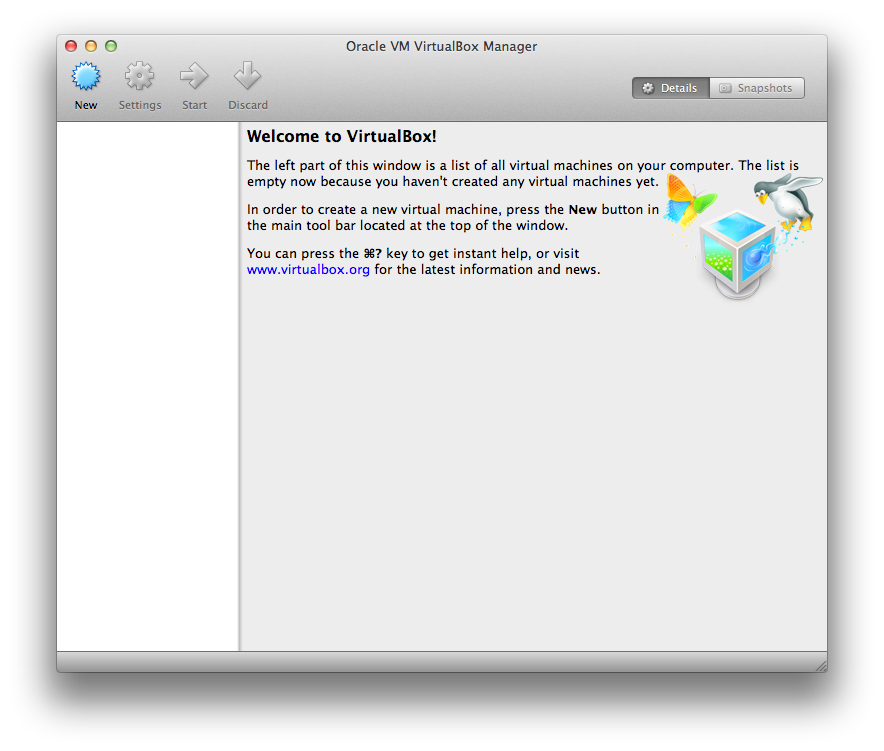
\includegraphics{VBox10_en_GB}}}
\caption{Start screen of Oracle VM VirtualBox.}
\label{VBox10}
\end{figure}

\section{Create a virtual machine}
In order to create a virtual machine, click on \command{New} in the VirtualBox program. In the following dialogue, you can name your machine, e.\,g. \command{IMAGINARY Entdeckerbox}, and choose type (\command{Linux}) und version (\command{Ubuntu (64\, bit)}) of the system that should run later on. The next step is to choose the size of the internal memory that will be allocated to the virtual machine. The size should not come below 1\, GB, but a bit more doesn't hurt. The next step deals with the creation of a virtual hard drive. Since we want to boot directly from DVD, we can choose \command{Do not add a virtual hard drive} and continue. The newly created virtual machine shows up in the list on the left. This process can be graphically understood in \cref{VBox20to50}. 
\begin{figure}[h]
\centering
\gfxscalebox{\smallshadow{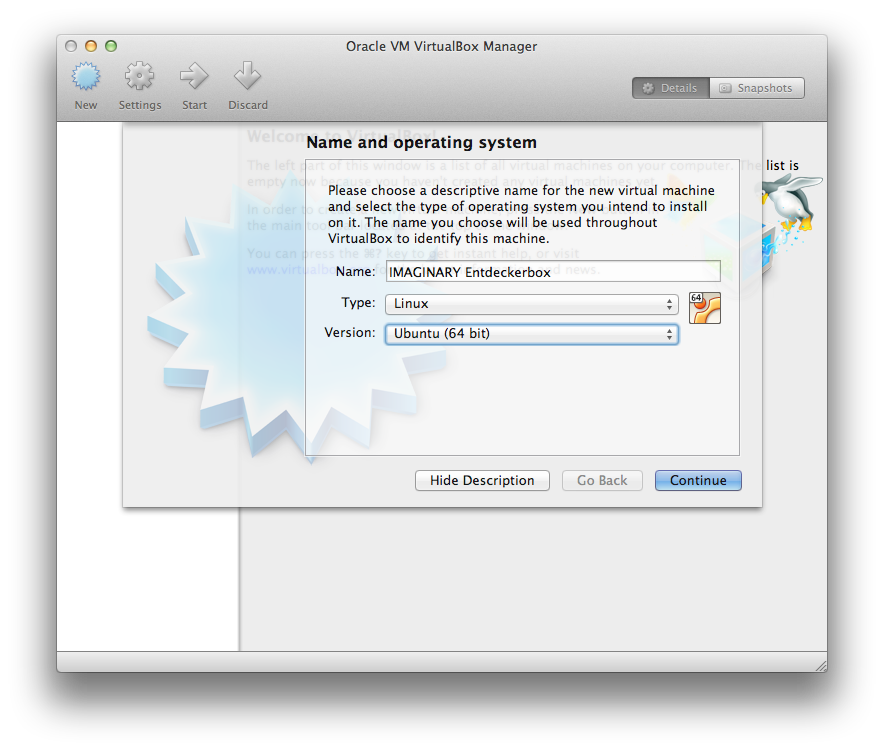
\includegraphics{VBox20_en_GB}}}
\qquad
\gfxscalebox{\smallshadow{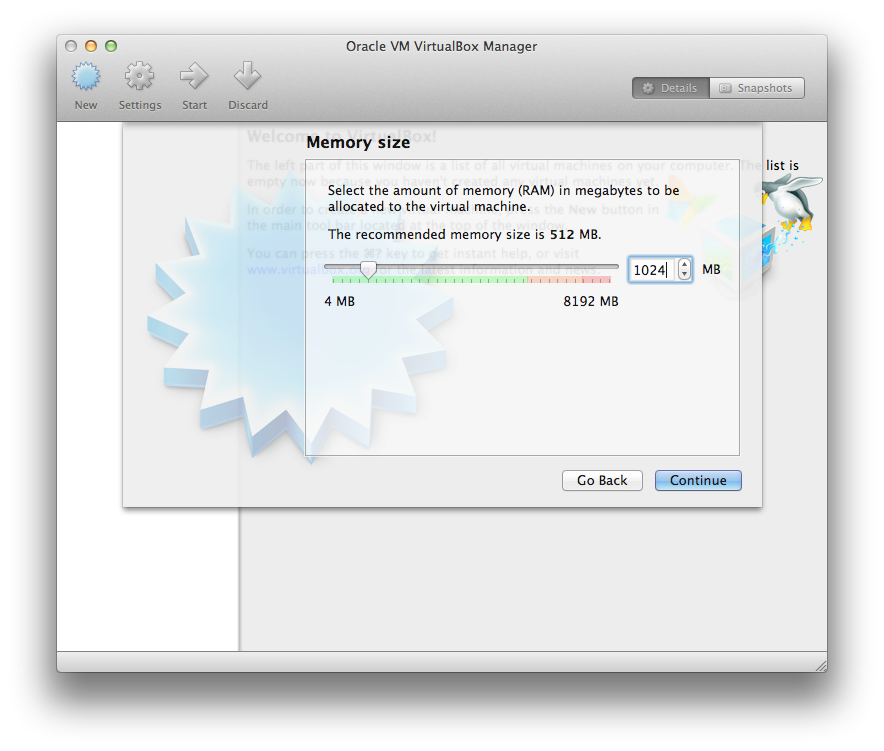
\includegraphics{VBox30_en_GB}}}
\\[\bigskipamount]
\gfxscalebox{\smallshadow{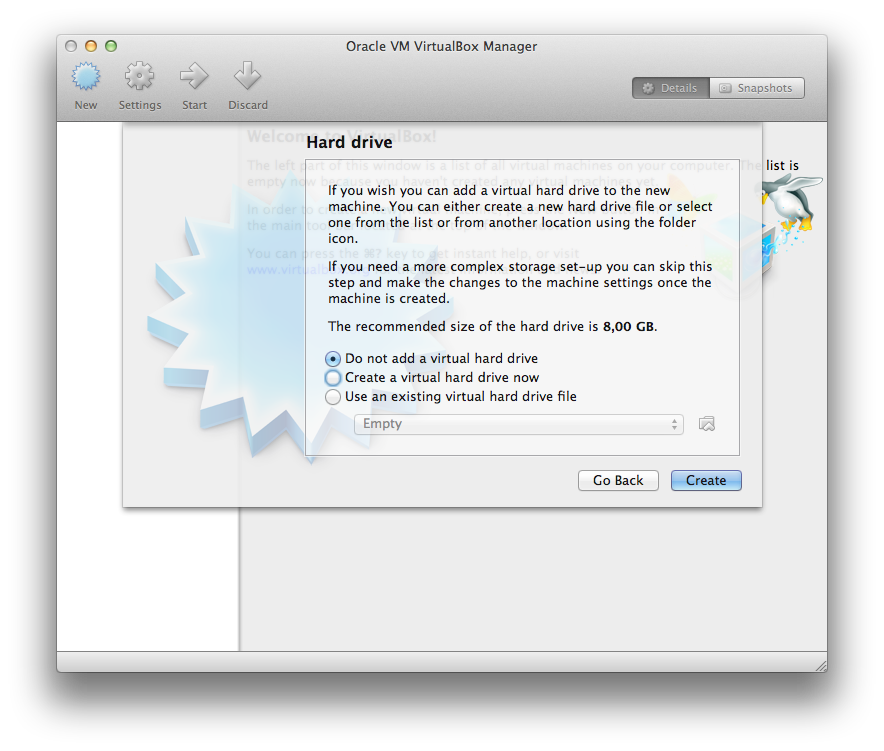
\includegraphics{VBox40_en_GB}}}
\qquad
\gfxscalebox{\smallshadow{\includegraphics{VBox50_en_GB}}}
\caption{Steps to create the virtual machine.}
\label{VBox20to50}
\end{figure}

Since some of the programs on the live DVD perform elaborate calculations, it is advisable to allocate more processing power to the virtual machine. For this purpose, choose the machine \command{IMAGINARY Entdeckerbox} from the list and click on \command{Settings}. The menu item \command{System} $\rightarrow$ \command{Processor} lets you choose the number of processors (\command{CPUs}) the virtual machine uses. Within the green range, the number should be as high as possible. In \cref{VBox60}, 8 out of 16 available processors were selected. It is not advisable to choose a number in the red range. If you'd like, you can experiment with the settings in order to obtain the best performance. The video card settings can be found under \command{Display}. You should allocate some graphics memory to the virtual machine and enable the 3d acceleration as shown in \cref{VBox60}. 
\begin{figure}[h]
\centering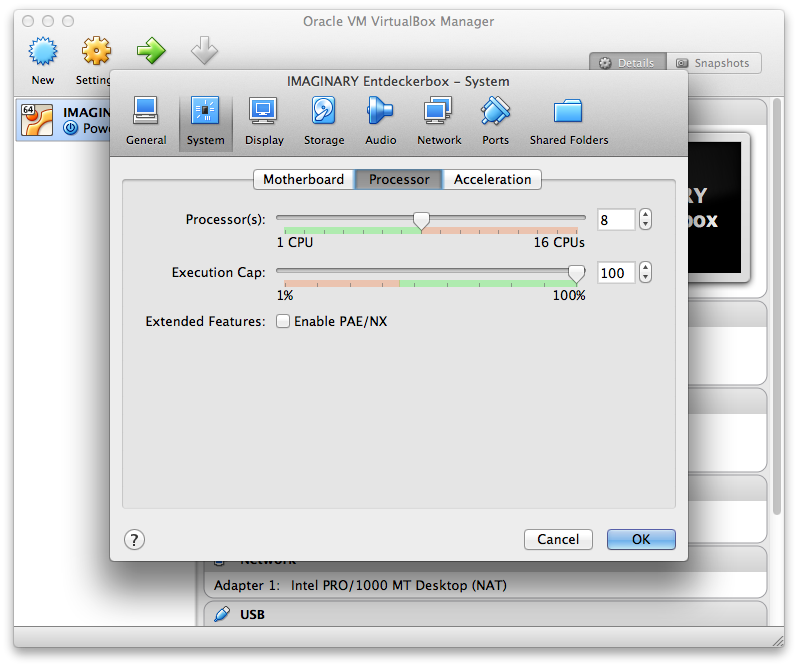
\includegraphics[scale=\gfxscale]{VBox60_en_GB}
\qquad\includegraphics[scale=\gfxscale]{VBox61_en_GB}
\caption{About half of the available processors should be allocated to the virtual machine. Also, you should increase the graphics memory and enable the 3d acceleration.}
\label{VBox60}
\end{figure}

\section{Launching the Entdeckerbox live DVD}
Before launching the virtual machine, you have to make sure that it actually uses the Entdeckerbox DVD. The virtual DVD drive needs to access the physical DVD drive of your computer. You can change this under \command{Settings} $\rightarrow$ \command{Storage}, as shown in \cref{VBox70}. Please note that the name of your DVD drive showing up behind \command{Host Drive} may be different from the name shown in \cref{VBox70}. Finally, activate the check box \command{Live CD/DVD} and close the dialogue window by clicking on \command{OK}.
\begin{figure}[h]
\centering\scalebox{\gfxscale}{\hspace{312px}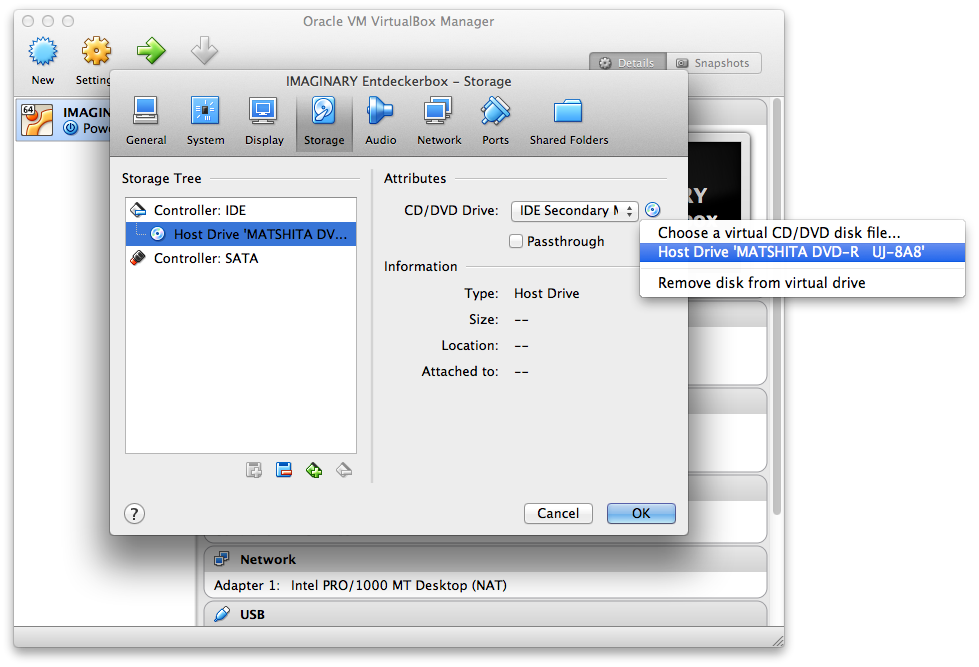
\includegraphics{VBox70_en_GB}}
\caption{Inserting the Entdeckerbox DVD into the virtual DVD drive.}
\label{VBox70}
\end{figure}

Congratulations! Now everything is set up and you can launch the virtual machine for the first time. By clicking onto the green \command{Start???} arrow, you can boot the system. This should look as in \cref{VBox8090}. 

As you can see, the live DVD runs in window mode. You can change the mode to \command{Full screen} by clicking on \command{View} in the menu of the running virtual machine. Since the programs of the Entdeckerbox DVD do not repsond to these changes in real time, you need to restart them. In the Entdeckerbox menu, for instance, you can change the resoultion by simply hitting \command{ESC}. 

\begin{figure}[h]
\centering
\gfxscalebox{\smallshadow{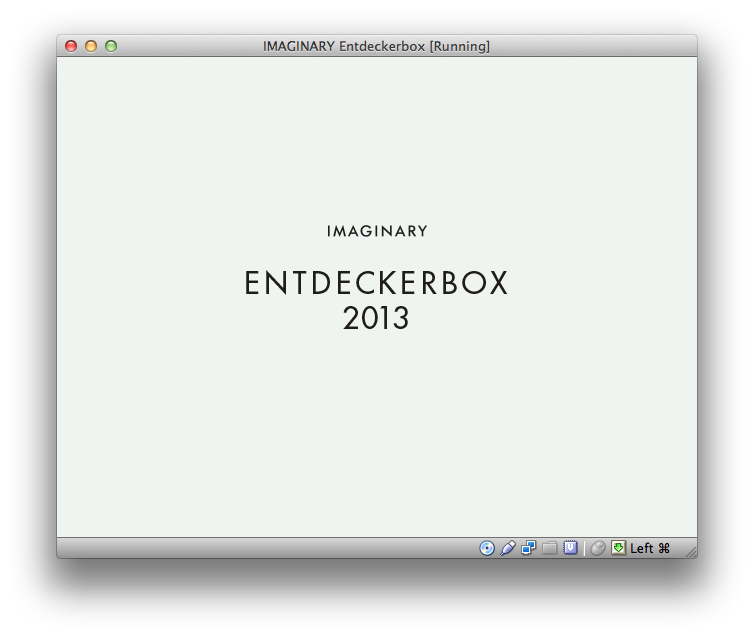
\includegraphics{VBox80}}}
\qquad
\gfxscalebox{\smallshadow{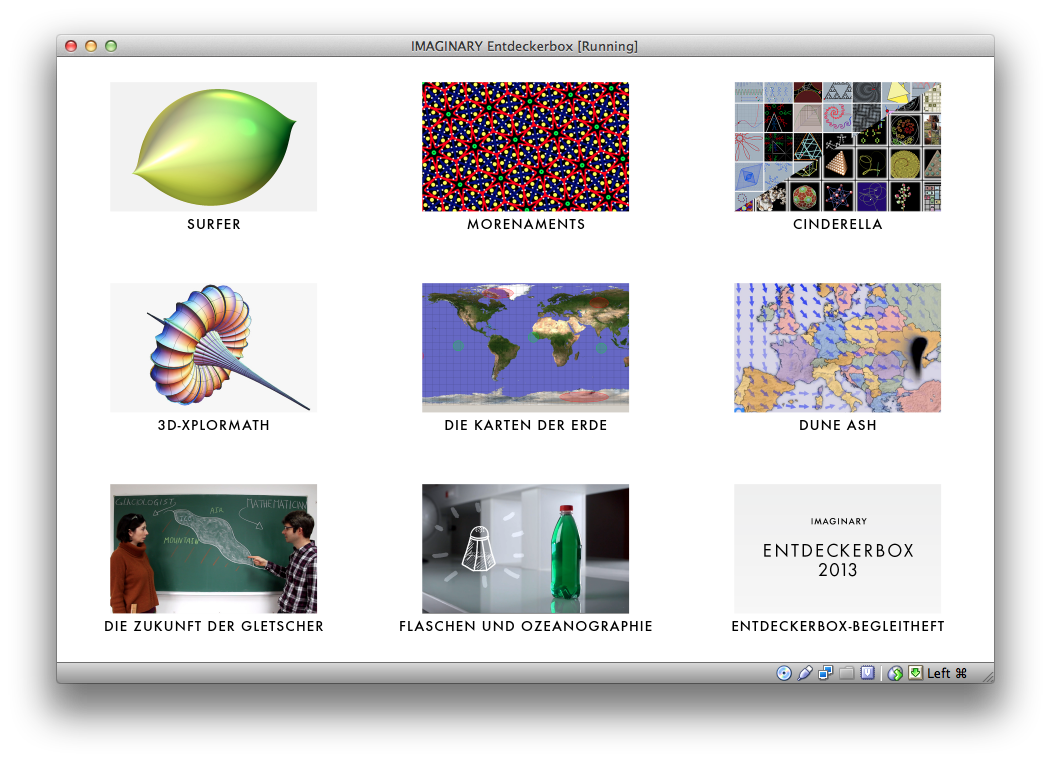
\includegraphics{VBox90}}}
\caption{A while after launching the virtual machine (left), the Entdeckerbox menu shows up (right).}
\label{VBox8090}
\end{figure}

\section{Trouble shooting}
\subsection{I have a 32\,bit operating system, and the live system does not launch!}
Since the live DVD runs with a 64\,bit operating system, a 64\,bit processor is expected. However, VirtualBox can access this from your 32\,bit operating system as long as your processor supports the so-called hardware virtualization. This is the case for pretty much all new processors, although it sometimes needs to be enabled manually in the BIOS. The label of this function differs, depending on the manufacturer (e.\,g. Intel Virtualization Technology, Intel VT-x, Virtualization Extensions, Intel VT-d, AMD-V or AMD IOMMU). 

\subsection{The launch of the live system takes a long time!}
The launch of a complete (albeit virtual) operating system does take some time. It can be drastically reduced though by creating an ISO image of the live system on your hard drive. Depending on the version of the live system (DVD or USB stick), you can find such an ISO image in the same folder as this manual or you have to create it yourself. The required programs are avaiable on the internet for free, for some operating systems they are already included. It is important to create an ISO image on a medium that is noticeably faster than your DVD drive. Solid-state drives are particularly suitable for this purpose. 

The ISO image should now be inserted into the virtual DVD drive. To this end, click on \command{Choose a virtual CD/DVD disk file...} in the menu shown in \cref{VBox70} and choose the ISO image. 
\end{document} 
